\part{Klasifikace příznaků}

Nalézt korespondující dvojice pozorovaných a simulovaných svazků pouze pomocí směru svazků je prakticky nemožné. Proto se pokusíme využít další příznaky, které nám pomohou eliminovat nesprávné korespondence. Víme, že u pozorovaných svazků můžeme kromě směru určit zářivý tok a detekovat ocásky (kapitola \ref{sec:beam parameters}).   

Prozkoumáme parametry pozorovaných a simulovaných svazků s cílem navrhnout jednoduchý klasifikátor. Nalezení závislosti parametrů zjednoduší úlohu korespondence svazků.  
\vspace{4mm}

\section{Ground truth}

Abychom mohli hledat závislosti mezi parametry pozorovaných a simulovaných svazků, potřebujeme získat data s korespondujícími svazky. Toho dosáhneme tak, že ručně upravujeme množinu korespondencí a optimalizujeme náklon faset. Proces ručního přiřazování svazků ukončíme, když nalezneme dostatečně přesný sklon faset. Takto nalezené korespondence považujeme za správné.    

Ručně určené korespondence označujeme výrazem "\textit{ground truth}" podobně jako v oblasti strojového učení, kde slouží jako přesná data v trénovací množině pro určení statistických modelů. Použití výrazu "\textit{ground truth}" je ovšem v našem případě sporné, neboť určení množiny korespondencí závisí na osobě, která tato úlohu provádí. To, co v našem případě označujeme jako "\textit{ground truth}", je množina, o které se domníváme, že by měla obsahovat správné korespondence svazků, ale v našem případě nemůžeme s naprostou jistotou tvrdit, že tomu tak je. 

\section{Změna zářivého toku se změnou parametrů kamene}
\label{sec: zmena_tok }

	Chceme zjistit, jak je zářivý tok svazků závislý na změně parametrů faset. 

	Máme k dispozici korespondující svazky z měření 10-ti různých kamenů typu \textit{viva12}. Při určení "\textit{ground truth}" jsme zároveň odhadli skutečné sklony faset a matematické modely kamenů. Vezmeme si postupně každý z těchto modelů a měníme náklon normály vybrané fasety o jeden stupeň ve čtyřech kolmých směrech. Nakonec normálu vrátíme zpět na původní hodnotu. Takto nakloníme normály všech 14-ti faset kamene. Dostaneme 4$\times$14 modelů kamene plus jeden původní. 
	
	Nakloněním normály fasety vznikne nový model kamene. Pro tento model pomocí LADOKu  vypočítáme parametry svazků. Pokud se zářivý tok svazku od původního modelu změnil, zapamatujeme si jeho hodnotu. Pro jednotlivý svazek dostaneme vektor hodnot zářivého toku $\vv{\phi}_e$. 
	
	 Abychom mohli porovnat změnu zářivého toku, který se může u svazků řádově lišit, vyjádříme změnu toku pomocí variačního koeficientu $c_v$. Variační koeficient je výsledkem podílu směrodatné odchylky a střední hodnoty vektoru $\vv{\phi}_e$. 
	 
	 \begin{equation}	 
	 c_v = \frac{\sigma(\vv{\phi}_e)}{E(\vv{\phi}_e)}\,. 
	 \end{equation}
	 
Určíme variační koeficient simulovaných svazků a výsledek ze všech 10-ti kamenů zaneseme do histogramu na obr. \ref{fig: flux_var_coeff}. V histogramu vidíme, že existuje nezanedbatelný počet svazků, pro které změna náklonu fasety o \SI{1}{\degree} znamená změnu zářivého toku o více než polovinu původní hodnoty. Je zřejmé, že obdobně se bude měnit zářivý tok svazků při posunu fasety. 

 Výsledek naznačuje, že nebude snadné nalézt funkci, která by definovala vztah mezi zářivým tokem simulovaných a pozorovaných svazků.  

\begin{figure}[htps]
\centering
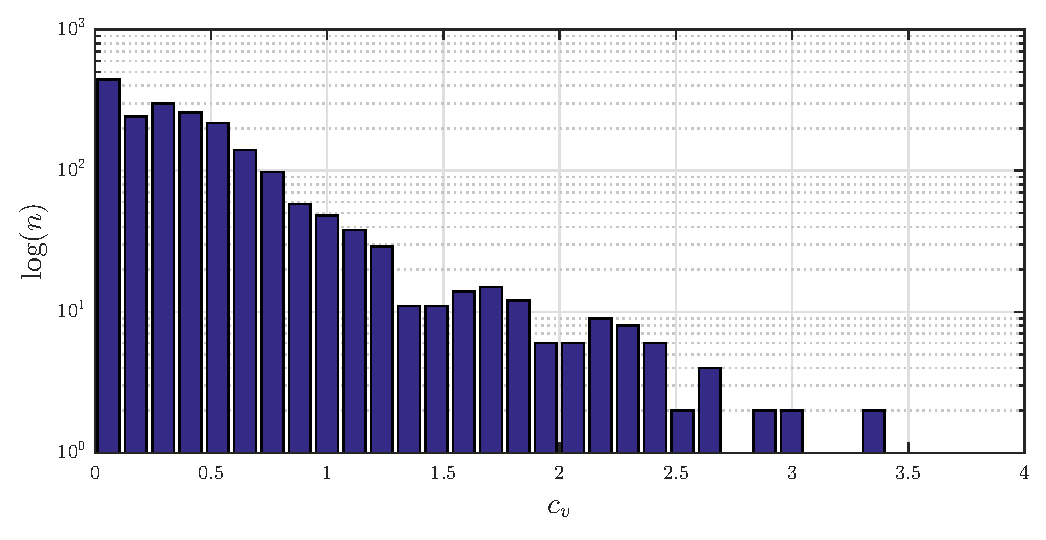
\includegraphics[width = 0.8\textwidth]{flux_var_coeff.eps}
\caption{Histogram variačního koeficientu zářivého toku svazků pro data z 10-ti snímků různých kamenů typu \textit{viva12}.}
\label{fig: flux_var_coeff}
\end{figure}



\section{Závislost zářivého toku}
\label{sec: tok_zavislost}
	Broušený kámen je ozářen laserovým svazkem o vlnové délce \SI{670}{\nano\metre}. Při průchodu světelného svazku kamenem se část záření absorbuje a přemění se na teplo. Absorpce záření závisí na odstínu kamene, proto si vybereme kameny stejného odstínu. V našem případě zvolíme odstín \textit{Hyacint}, který se vyznačuje nízkou absorpcí zdrojového svazku. 
	
	Korespondující svazky jsme určili pro 4 kameny odstínu \textit{Hyacint}, kde každý kámen byl 3$\times$ s různou rotací umístěn do měřicí soustavy. S korespondencemi z 12 snímků pracujeme jako s celkem a dostaneme množinu uspořádaných dvojic pozorovaných a simulovaných svazů. 
	
	Pozorované svazky charakterizuje zářivý tok $\vv{\phi}_{e_m}$ a simulované svazky zářivý tok $\vv{\phi}_{e_r}$. Cílem je nalézt funkci $h$, pro kterou
	
	\begin{equation}	
		\phi_{e_r} = h \left( \phi_{e_m} \right) \,.
		\label{eq: fi_fi}
	\end{equation}

Abychom mohli porovnat data z více měření, vyjádříme si zářivý tok pozorovaných svazků jako jejich poměr ku součtu zářivého toku všech pozorovaných svazků v jednotlivém snímku. 

Závislost $\phi_{e_r} =  f\left( \phi_{e_m} \right)$ vyneseme do grafu na obr. \ref{fig: flux_depend2}, kde jsou vykresleny pouze svazky s variačním koeficientem $c_v$ menším než $0.5$.

\begin{figure}[htps]
\centering
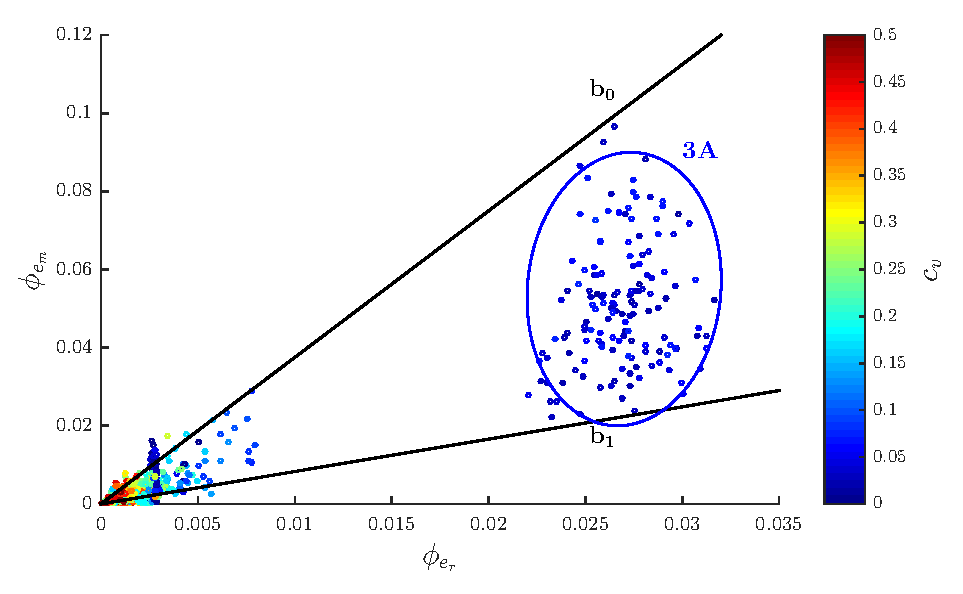
\includegraphics[width = 0.8\textwidth]{flux_depend2.eps}
\caption[Závislost zářivého toku simulovaných a pozorovaných svazků.]{Závislost velikosti zářivého toku simulovaných svazků na velikosti zářivého toku pozorovaných svazků. Zobrazeny jsou pouze svazky s variačním koeficientem zářivého toku větším než $0.5$. Výsledky pro odstín \textit{Hyacint}. Vynechány jsou svazky třídy \textbf{3B}. Přímky $\mathbf{b_0}$ a $\mathbf{b_1}$ naznačují, že rozptyl zářivého toku pozorovaných svazků roste s velikostí zářivého toku simulovaných svazků. Svazky třídy \textbf{3A} jsou zvýrazněny.}
\label{fig: flux_depend2}
\end{figure}

\begin{figure}[htps]
\centering
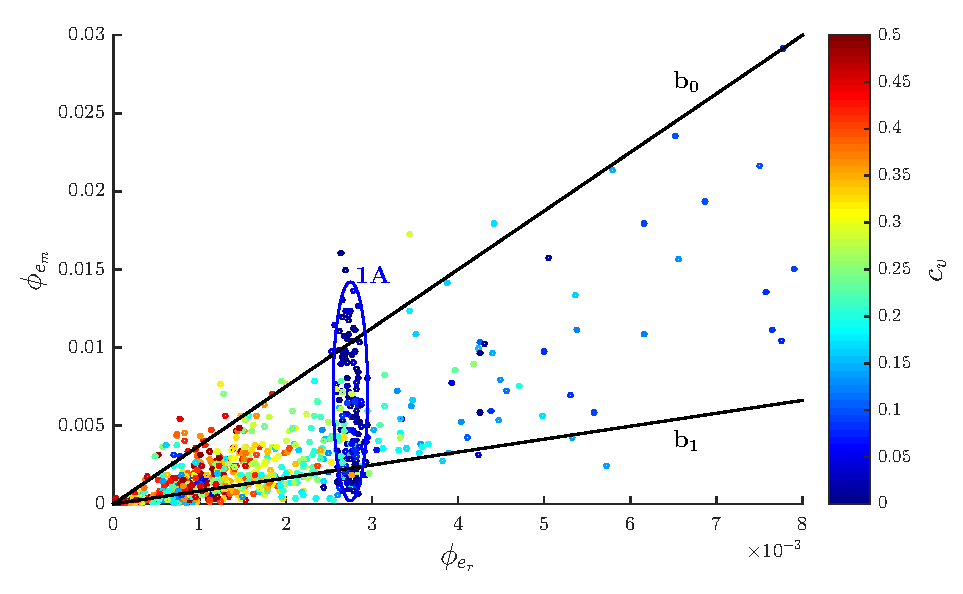
\includegraphics[width = 0.8\textwidth]{flux_depend1.eps}
\caption[Závislost zářivého toku simulovaných a pozorovaných svazků - detail.]{Detail obrázku \ref{fig: flux_depend2}. Vynechány jsou svazky třídy \textbf{3A} a \textbf{3B}. Svazky třídy \textbf{1A} jsou zvýrazněny.}
\label{fig: flux_depend1}
\end{figure}

  Výsledek není příliš optimistický. Data v grafu jsou příliš rozptýlena na to, abychom mohli nalézt spolehlivou funkci popisující závislost \ref{eq: fi_fi}. Důvodů může být hned několik. 

Víme, že v modelu kamene nejsou postihnuty všechny skutečnosti ovlivňující velikost zářivého toku stop. Můžeme zmínit například to, že v modelu není zahrnuta čistota materiálu, která nemusí a prakticky ani není v celém materiálu konstantní. Nedokonalé proleštění fasety ovlivňuje rozptylové parametry světelného svazku. Změna parametrů fasety vede ke změně plochy fasety, tedy i ke změně plochy svazku, který je omezen hranou této fasety. Malá změna parametrů fasety může vést k velké změně zářivého toku svazku, což jsme si ukázali v kapitole \ref{sec: zmena_tok }. Tyto a další vlastnosti v konečném důsledku vyústí v chybu údaje na y-ové ose grafu \ref{fig: flux_depend2}.

Na druhé straně musíme počítat s nejistotou určení zářivého toku pozorovaných svazků vznikající při výpočtu parametrů svazků z obrazu. Mezi zásadní problémy patří šum, překrývání stop, difuzní odrazivost svazků či odhad pozadí snímku.  


\section{Závislost parametrů ocásků}

	Zajímáme se o to, jak může přispět znalost ocásků pozorovaných a simulovaných svazků k nalezení korespondující dvojice.  

  Korespondující ocásky nalezeme pomocí jednoduchého algoritmu založeného na podobnosti směru ocásků korespondujících stop. Takto nalezené korespondence zkontrolujeme a případně upravíme. Máme k dispozici data korespondujících ocásků pro 25 snímků celkem deseti kamenů \textit{viva12}. 
	
	Ocásky parametrizujeme pomocí velikosti $\rho$ a směrového úhlu $\phi$. Z korespondujících ocásků získáme parametry pozorovaných ocásků $\vv{\rho}_m$ a $\vv{\varphi}_m$ a k nim odpovídající simulované parametry $\vv{\rho}_r$ a $\vv{\varphi}_r$.
	

\subsection{Směrový úhel}
 U směrového úhlu potřebujeme vědět, do jaké míry souhlasí směr pozorovaného a směr simulovaného ocásku. Vypočítáme rozdíl směrových úhlů $\Delta\vv{\phi}$ a vyneseme do grafu \ref{fig: tail_depend1} rozložení pravděpodobnosti.  
 
 \begin{equation}
 \Delta\vv{\phi} = \vv{\varphi}_m - \vv{\varphi}_r\,.
 \end{equation}
  
\begin{figure}[htps]
\centering
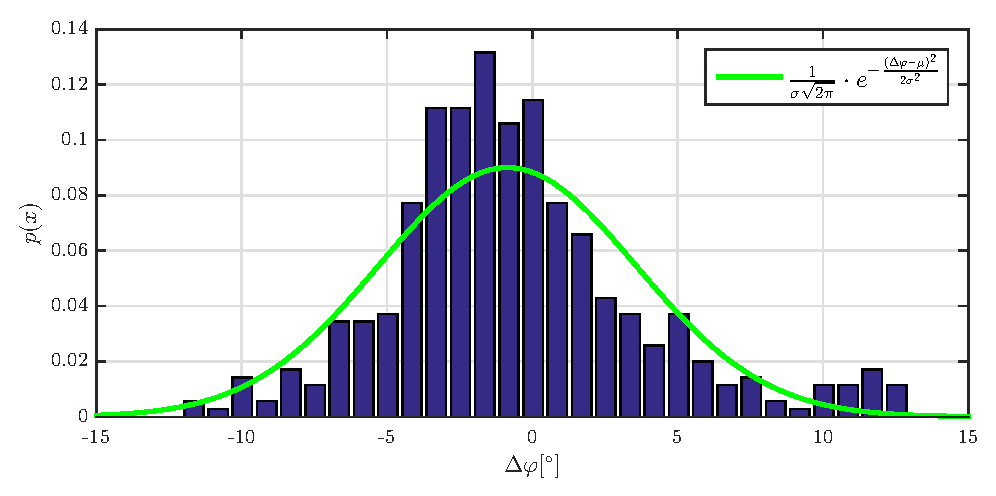
\includegraphics[width = 0.8\textwidth]{tails_gauss.eps}
\caption[Odhad pravděpodobnostní funkce rozdílu směrového úhlu mezi pozorovanými a simulovanými ocásky.]{Odhad pravděpodobnostní funkce rozdílu směrového úhlu mezi pozorovanými a simulovanými ocásky. Aproximace Gaussovou křivkou s parametry $\sigma = $ \SI{4.43}{\degree} a $\mu = $ \SI{-0.86}{\degree}. }
\label{fig: tail_depend1}
\end{figure}

Pravděpodobnostní rozdělení na obr. \ref{fig: tail_depend1} lze aproximovat Gaussovu funkcí

\begin{equation}
f(\Delta\varphi) = \frac{1}{\sigma\sqrt{2\pi}}\cdot e^{-\frac{\left(\Delta\varphi - \mu\right)^2}{2\sigma^2}}\, 
\end{equation}
s rozptylem $\sigma =  $ \SI{4.43}{\degree} = \SI{0.077}{\radian} a střední hodnotou $\mu = $ \SI{-0.86}{\degree} = \SI{-0.15}{\radian}. Tato funkce může sloužit jako základ pro určení podobnosti ocásků.   

\subsection{Velikost}
	Vykreslili jsme si závislost velikosti simulovaných ocásků na velikosti pozorovaných ocásků. Graf na obr. \ref{fig: tail_depend2} obsahuje pouze náhodně vybrané vzorky závislosti $\rho_r = f(\rho_m)$, kde $\rho_m~=~\dfrac{\rho_m}{max{\vv{\rho}_m}}$. Zdá se, že mezi velikostí pozorovaných a simulovaných ocásků není takřka žádná souvislost. Nejsme schopni nalézt funkci $f$, která by popisovala závislost $\rho_r = f(\rho_m)$.
	
	\begin{figure}[htps]
\centering
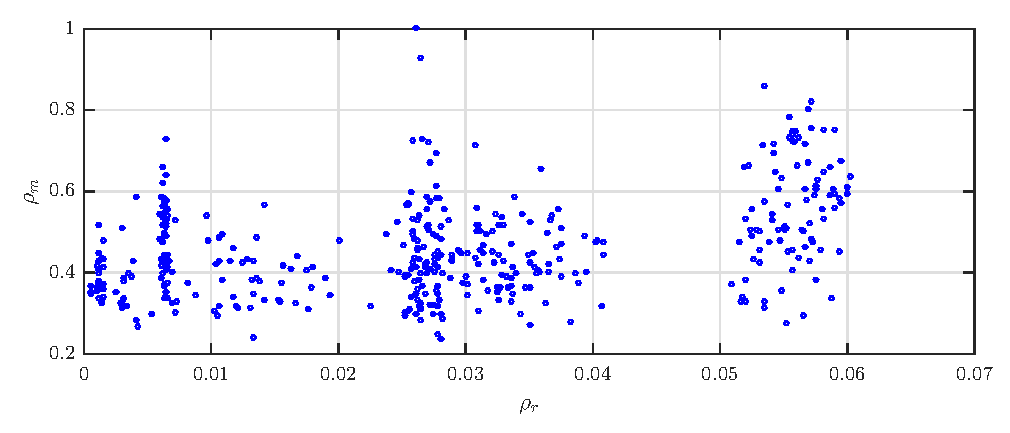
\includegraphics[width = 0.8\textwidth]{tails_rho.eps}
\caption[Závislost velikosti simulovaných a pozorovaných ocásků.]{Závislost velikosti simulovaných ocásků $\rho_r$ na velikosti pozorovaných ocásků $\rho_m$ pro náhodně vybranou podmnožinu korespondujících ocásků.}
\label{fig: tail_depend2}
\end{figure}

\clearpage